% CryptAgent BTP-II: idea, gap, and study design.
% Edit the three names and contribution statements before presenting.
\documentclass[aspectratio=169,10pt]{beamer}
\usetheme{Madrid}
\usecolortheme{default}
\usepackage[T1]{fontenc}
\usepackage{lmodern}
\usepackage{booktabs}
\usepackage{tabularx}
\usepackage{array}
\usepackage{tikz}
\usetikzlibrary{arrows.meta,positioning}
\definecolor{cryptblue}{HTML}{173B70}
\definecolor{cryptteal}{HTML}{0B7A78}
\setbeamercolor{structure}{fg=cryptblue}
\setbeamercolor{frametitle}{fg=white,bg=cryptblue}
\setbeamercolor{block title}{fg=white,bg=cryptteal}
\setbeamertemplate{navigation symbols}{}
\setbeamertemplate{footline}[frame number]
\newcommand{\ca}{CryptAgent}
\newcommand{\mone}{Member 1 (name)}
\newcommand{\mtwo}{Member 2 (name)}
\newcommand{\mthree}{Member 3 (name)}
\title[CryptAgent: BTP-II]{CryptAgent\\A study design for checking cryptographic integration code}
\subtitle{BTP-II: problem, evidence gap, and experimental plan}
\author[Three-member team]{\mone\\[0.2em]\mtwo\\[0.2em]\mthree}
\institute{Three-member BTP project team}
\date{\today}

\begin{document}
\begin{frame}\titlepage\end{frame}

\begin{frame}{BTP-II question and scope}
\begin{block}{Research question}
How can an assistant review a C++ cryptographic integration against explicit requirements, locate likely misuse, and say when evidence is insufficient?
\end{block}
\begin{itemize}
\item Focus for this course: motivation, gap, requirements, study design, and evaluation method.
\item Current fixed case: AES-128-GCM, C++20, Windows CNG, message tampering.
\item Early implementation feedback helped narrow this design; detailed implementation results belong in BTP-III.
\end{itemize}
\end{frame}

\begin{frame}{Why integration code is a useful target}
\begin{columns}[T]
\column{0.49\textwidth}
\begin{block}{Correct primitive}
AES-GCM provides encryption and authentication when its inputs and outputs are used correctly.
\end{block}
\column{0.49\textwidth}
\begin{alertblock}{Incorrect integration}
A wrapper can ignore decryption status, expose plaintext too early, reuse a nonce, or misstate a buffer length.
\end{alertblock}
\end{columns}
\vspace{0.6em}
\centering\large The security question concerns the \emph{application's use} of the API.
\end{frame}

\begin{frame}{Technical background: AES-GCM and CNG}
\begin{itemize}
\item GCM is authenticated encryption with associated data (AAD): the tag authenticates ciphertext and AAD.
\item This project profile fixes a 16-byte key, 12-byte nonce, and 16-byte tag.
\item Encryption nonces must not repeat under the same key; decryption must reject tag mismatch.
\item Windows CNG exposes \texttt{BCryptEncrypt}, \texttt{BCryptDecrypt}, and authenticated-mode parameters.
\end{itemize}
\vfill
{\scriptsize Basis: NIST SP 800-38D; Microsoft \texttt{BCryptDecrypt} and \texttt{BCRYPT\_AUTHENTICATED\_CIPHER\_MODE\_INFO} documentation.}
\end{frame}

\begin{frame}{Gap identification: a project-specific gap}
\begin{tabularx}{\textwidth}{>{\bfseries}p{2.5cm}X}
\toprule
Available guidance & What it supplies \\
\midrule
NIST SP 800-38D & The authenticated-encryption specification and security conditions. \\
Microsoft CNG docs & API parameters, output buffer semantics, and authentication status. \\
Our Phase 1--3 work & Threat model, contract, synthetic scenarios and evidence policy for an earlier profile. \\
\bottomrule
\end{tabularx}
\vspace{1em}
\begin{block}{Design gap}
We still need a profile-specific bridge from submitted C++ source to requirement-level, source-linked findings and explicit uncertainty. Documentation alone does not assess an arbitrary wrapper.
\end{block}
\end{frame}

\begin{frame}{Precise problem statement}
\begin{enumerate}
\item Accept one C++ source excerpt or file for a \emph{fixed} Windows CNG AES-GCM profile.
\item Determine whether the code is in scope and which relevant context is visible.
\item Review five requirements; cite actual source lines for concerns.
\item Separate an observation or model opinion from a confirmed runtime witness.
\item Return ``insufficient context'' or ``review unavailable'' when support is missing.
\end{enumerate}
\vspace{0.4em}
\alert{The study does not assume that an LLM's confident statement is ground truth.}
\end{frame}

\begin{frame}{Threat model and fixed profile}
\begin{columns}[T]
\column{0.5\textwidth}
\textbf{Attacker can:}
\begin{itemize}
\item Modify encrypted inputs, including ciphertext, nonce, tag or AAD.
\item Observe public status and output.
\end{itemize}
\column{0.5\textwidth}
\textbf{Assumptions / exclusions:}
\begin{itemize}
\item Secret key is unavailable to the attacker; OS and CNG are trusted.
\item Replay prevention, physical leakage and universal memory-safety proofs are outside this study.
\end{itemize}
\end{columns}
\vspace{0.4em}
\begin{block}{Reason for fixing the choices}
One profile keeps data labels, prompts, checks and outcome comparisons consistent.
\end{block}
\end{frame}

\begin{frame}{Five planned review requirements}
\small
\begin{tabularx}{\textwidth}{>{\bfseries}p{1.15cm}X}
\toprule
ID & Requirement and evidence question \\
\midrule
F01 & Functional correctness: do supported messages encrypt and decrypt correctly? \\
F02 & Tampering rejection: are modified protected inputs rejected? \\
F03 & Authentication before output: can failure expose plaintext or report success? \\
F04 & Key, nonce and tag handling: correct profile sizes and no nonce reuse under one key? \\
F05 & Input/output boundaries: safe length checks, casts and buffer capacities? \\
\bottomrule
\end{tabularx}
\end{frame}

\begin{frame}{Proposed study design}
\centering
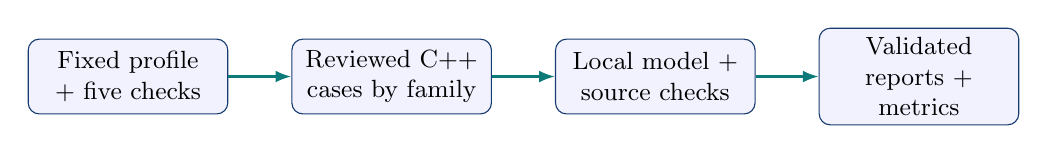
\begin{tikzpicture}[node distance=0.9cm and 0.8cm, every node/.style={font=\small},
 box/.style={draw=cryptblue,rounded corners,fill=blue!5,minimum height=0.95cm,text width=2.3cm,align=center},
 arr/.style={-{Latex[length=2mm]},thick,draw=cryptteal}]
\node[box] (contract) {Fixed profile + five checks};
\node[box,right=of contract] (cases) {Reviewed C++ cases by family};
\node[box,right=of cases] (review) {Local model + source checks};
\node[box,right=of review] (score) {Validated reports + metrics};
\draw[arr] (contract)--(cases); \draw[arr] (cases)--(review); \draw[arr] (review)--(score);
\end{tikzpicture}
\vspace{1.2em}
\begin{itemize}
\item Ground labels in actual code and cited lines; retain ``insufficient context'' cases.
\item Keep implementation families together when making train/development/test splits.
\item Use native Windows CNG tests for stronger evidence when a suitable machine exists.
\end{itemize}
\end{frame}

\begin{frame}{Expansion after the controlled AES profile}
\small
\begin{tabularx}{\textwidth}{>{\bfseries}p{2.5cm}p{3.2cm}X}
\toprule
Profile & Language / library & Profile-specific study question \\
\midrule
AES-128-GCM & C++20 / Windows CNG & Authentication, nonce and boundary handling. \\
CKKS & Python / TenSEAL & Secret-key and result boundaries; input contracts. \\
TFHE & Rust / TFHE-rs & Key roles, result boundaries and numeric limits. \\
BFV & C++20 / OpenFHE & Lattice-based key and plaintext-domain boundaries. \\
\bottomrule
\end{tabularx}
\vspace{0.7em}
\alert{The midterm studies verification only. Each profile needs its own requirements and labels; selectable schemes and generation are later goals.}
\end{frame}

\begin{frame}{How success will be measured}
\begin{itemize}
\item \textbf{Output validity:} correct JSON, five IDs, real source quotations and valid line numbers.
\item \textbf{Security classification:} per-check true positives, false positives and missed issues.
\item \textbf{Location/explanation:} does the cited line support the stated concern?
\item \textbf{Uncertainty:} does the system abstain on partial or out-of-scope code?
\item \textbf{Later runtime evidence:} native CNG tests with synthetic messages and tampered inputs.
\end{itemize}
\vspace{0.3em}
\alert{Report raw counts and limitations; avoid inferring generalization from related synthetic variants.}
\end{frame}

\begin{frame}{Early feedback that refined the design}
\begin{itemize}
\item The earlier Phase 1--3 profile used libsodium/XChaCha20-Poly1305 and a broader contract; its 150 synthetic cases share 30 scenario groups.
\item The current work therefore narrowed the active midterm study to one AES/CNG profile and five checks.
\item Early local-model trials showed that schema-valid output and cryptographic accuracy are different questions.
\item The revised design requires explicit source evidence, non-verdict states and a fresh held-out evaluation set.
\end{itemize}
\vfill
{\scriptsize BTP-II takeaway: this slide motivates the revised method; full implementation outcomes are presented in BTP-III.}
\end{frame}

\begin{frame}{Three-member plan and individual contributions}
\small
\begin{tabularx}{\textwidth}{>{\bfseries}p{2.7cm}X}
\toprule
Team member & Replace with the member's \emph{actual} BTP-II contribution \\
\midrule
\mone & Problem framing, literature/gap analysis, or threat-model work: \textbf{[edit to actual contribution]}. \\
\mtwo & Requirements and experimental protocol: \textbf{[edit to actual contribution]}. \\
\mthree & Dataset/evaluation design and feasibility study: \textbf{[edit to actual contribution]}. \\
\bottomrule
\end{tabularx}
\vspace{0.6em}
{\scriptsize These are editable prompts, not assertions about who did what. Add concrete files, decisions and evidence for each member.}
\end{frame}

\begin{frame}{BTP-II conclusion and next steps}
\begin{block}{Study proposal}
Evaluate whether a local assistant can turn AES/CNG source into requirement-level, source-linked reviews while preserving uncertainty.
\end{block}
\begin{enumerate}
\item Independently review full-session labels and collect diverse CNG implementations.
\item Freeze a fresh test set before model tuning.
\item Compare a base-model baseline with a fine-tuned adapter.
\item Add native Windows CNG checks for confirmed functional/tampering evidence.
\end{enumerate}
\end{frame}

\begin{frame}{References}
\scriptsize
\begin{thebibliography}{9}
\bibitem{nist} NIST, \emph{SP 800-38D: Galois/Counter Mode (GCM) and GMAC}, 2007. \url{https://csrc.nist.gov/pubs/sp/800/38/d/final}
\bibitem{dec} Microsoft, \emph{BCryptDecrypt function}. \url{https://learn.microsoft.com/en-us/windows/win32/api/bcrypt/nf-bcrypt-bcryptdecrypt}
\bibitem{auth} Microsoft, \emph{BCRYPT\_AUTHENTICATED\_CIPHER\_MODE\_INFO}. \url{https://learn.microsoft.com/en-us/windows/win32/api/bcrypt/ns-bcrypt-bcrypt_authenticated_cipher_mode_info}
\bibitem{local} CryptAgent repository: \texttt{phase1/}, \texttt{STATUS.md}, \texttt{profiles/aes128\_gcm\_tampering.json} (local project artifacts).
\end{thebibliography}
\end{frame}
\end{document}
